\section{Пример работы}

Будем использовать простой декоратор
для вывода состояния дерева до
и после выполнения примера:

\begin{lstlisting}
examples = []


def example(name):
    def decorator(f):
        def wrapper(t):
            print(f'Example {name}:')
            print(f'Original tree: {t}')

            f(t)

            print('Tree:')
            t.print_tree()
        examples.append(wrapper)
        return wrapper
    return decorator
\end{lstlisting}

\subsection{Поиск}

Код примера:

\begin{lstlisting}
@example('find')
def example_find(t):
    for k in t:
        print(f'{k}: {t.find(k)}')
\end{lstlisting}

Результат выполнения примера (рис. \ref{fig:find}):

\begin{figure}[H]
    \centering
    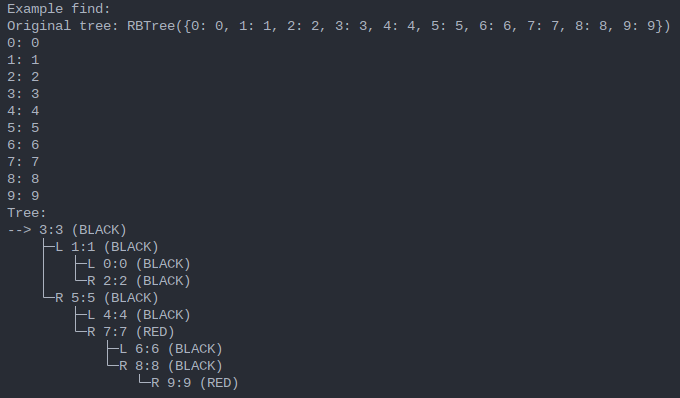
\includegraphics[width=0.85\linewidth]{photo/example_find}
    \caption{Результат выполнения операции "поиск"}
    \label{fig:find}
\end{figure}

\subsection{Вставка}

Код примера:

\begin{lstlisting}
@example('insert')
def example_insert(t):
    t.insert(1, 'new_value')
    print('Replaced value at key 1 with "new_value":')
    print(t)
    
    t.insert('new_key', 'another_value')
    print('Inserted value "new_value" with key "new_key":')
    print(t)
\end{lstlisting}

Результат выполнения примера (рис. \ref{fig:insert}):

\begin{figure}[H]
    \centering
    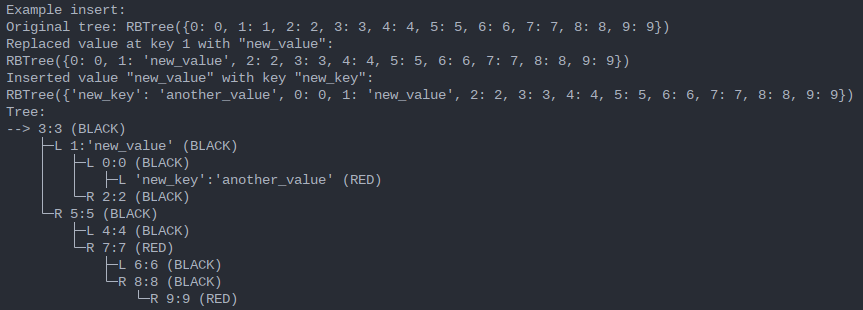
\includegraphics[width=0.85\linewidth]{photo/example_insert}
    \caption{Результат выполнения операции "вставка"}
    \label{fig:insert}
\end{figure}

\subsection{Удаление}

Код примера:

\begin{lstlisting}
@example('remove')
def example_remove(t):
    print('Removed key 7:')
    t.remove(7)
    print(t)
\end{lstlisting}

Результат выполнения примера (рис. \ref{fig:remove}):

\begin{figure}[H]
    \centering
    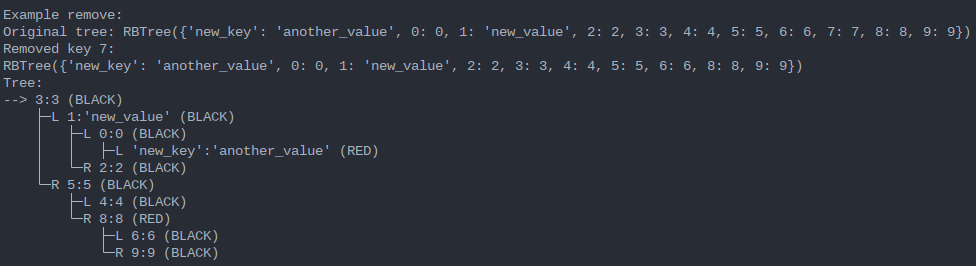
\includegraphics[width=0.85\linewidth]{photo/example_remove}
    \caption{Результат выполнения операции "удаление"}
    \label{fig:remove}
\end{figure}

\subsection{Получение ключей/значений}

Код примера:

\begin{lstlisting}
@example('keys and values')
def example_keys_and_values(t):
    print('Keys:')
    print(t.get_keys())
    
    print('Values:')
    print(t.get_values())
\end{lstlisting}

Результат выполнения примера (рис. \ref{fig:kv}):

\begin{figure}[H]
    \centering
    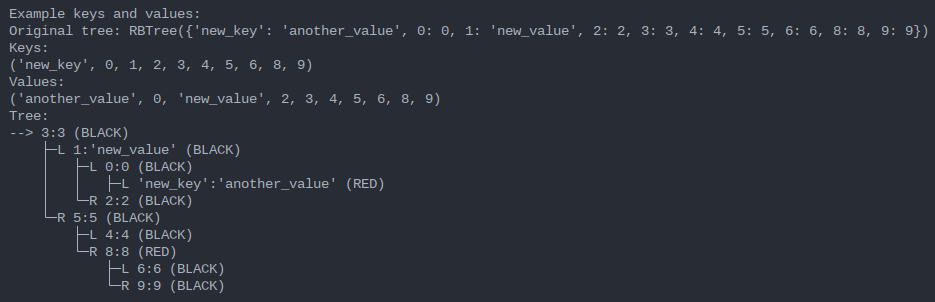
\includegraphics[width=0.85\linewidth]{photo/example_kv}
    \caption{Результат выполнения операции "получение ключей/значений"}
    \label{fig:kv}
\end{figure}
